\documentclass{article}
\usepackage{setspace}
\usepackage{geometry}
\usepackage[utf8]{inputenc}
\usepackage{amsmath,amsthm,amssymb,bm}
\usepackage{mathtools}

\geometry{letterpaper, portrait, margin=1in}
\setstretch{1.5}
\title{Homework 10}
%\date{1-18-2020}
\author{Runmin Lu}

\begin{document}
	\maketitle
	%\newpage
	
	\section*{Exercise 6.1}
	\subsection*{(a)}
		For small positive $\varepsilon$ and vectors in $\mathbb R^2$,\\
		$\varepsilon(1, 0)^T$ and $\varepsilon(-1, 0)^T$ have high Euclidean distance similarity: $d = 2\varepsilon \approx 0$ but low cosine similarity $-1$.\\
		For large positive $K$,\\
		$\frac K{\sqrt{1 - \cos\varepsilon}}(1, 0)^T$ and $\frac K{\sqrt{1 - \cos\varepsilon}}(\cos\varepsilon, \sin\varepsilon)^T$ have high cosine similarity: $\cos \varepsilon \approx 1$ but low Euclidean distance similarity: $d = \frac K{\sqrt{1 - \cos\varepsilon}}\sqrt{(\cos\varepsilon-1)^2 + \sin^2\varepsilon} = K\sqrt 2$
			
	\subsection*{(b)}
		Cosine similarity changes because for any pair of points with small Euclidean distance, if you move the origin to their midpoint, then CosSim $= -1$ but Euclidean distance won't change because when computing the norm of their difference, the shifted amount cancel out for each component.\\
		Therefore, when using Cosine similarity, we need to properly place the origin for it to work well.
		
	\section*{Exercise 6.2}
		\begin{align*}
			\mathbb P[f(\mathbf x) \neq y] &=
			\begin{cases}
				\mathbb P[y = -1 | \mathbf x] = 1 - \pi(\mathbf x)   &\text{if } f(\mathbf x) = +1 \rightarrow \pi(\mathbf x) \geq \frac12\\
				\mathbb P[y = +1 | \mathbf x] = \pi(\mathbf x) &\text{if } f(\mathbf x) = -1 \rightarrow \pi(\mathbf x) < \frac12
			\end{cases}\\
			\text{When } \pi(\mathbf x) &\geq \frac12:\\
			1 - \pi(\mathbf x) &< \frac12 \leq \pi(\mathbf x)\\
			\text{When } \pi(\mathbf x) &< \frac12:\\
			\pi(\mathbf x) &< \frac12 \leq 1 - \pi(\mathbf x)\\
			\mathbb P[f(\mathbf x) \neq y] &=\min(\pi(\mathbf x), 1 - \pi(\mathbf x))
		\end{align*}
		For other hypothesis $h$,
		\begin{align*}
			e(h(\mathbf x)) &= \mathbb P[h(\mathbf x) = +1, y = -1|\mathbf x] + \mathbb P[h(\mathbf x) = -1, y = +1|\mathbf x]\\
			&= \mathbb P[h(\mathbf x) = +1](1 - \pi(\mathbf x)) + (1 - \mathbb P[h(\mathbf x) = +1])\pi(\mathbf x)\\
			&\text{for simplicity, let } p = \mathbb P[h(\mathbf x) = +1]\\
			e(h(\mathbf x)) &= p(1 - \pi(\mathbf x)) + (1 - p)\pi(\mathbf x)
		\end{align*}
		This is a function of $p$ defined in $[0, 1]$, which takes value $\pi(\mathbf x)$ at $p = 0$ and $1-\pi(\mathbf x)$ at $p = 1$. This function is also linear so the optimum value can only be on the boundary of the domain so the minimum is $\min(\pi(\mathbf x), 1 - \pi(\mathbf x)) = e(f(\mathbf x))$
		
	\section*{Problem 6.1}
		Note: blue is $+1$ and red is $-1$. Fuzzy boundaries are resulted from randomized tie breaking algorithm.
	\subsection*{(a)}
		1-NN:\\
		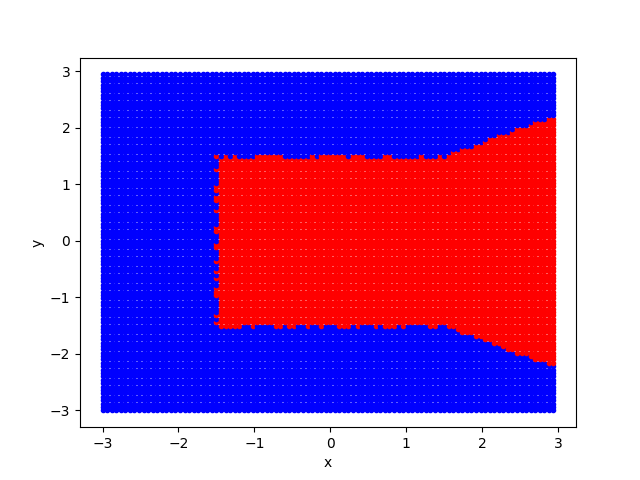
\includegraphics[scale=0.8]{p6.1a1}\\
		3-NN:\\
		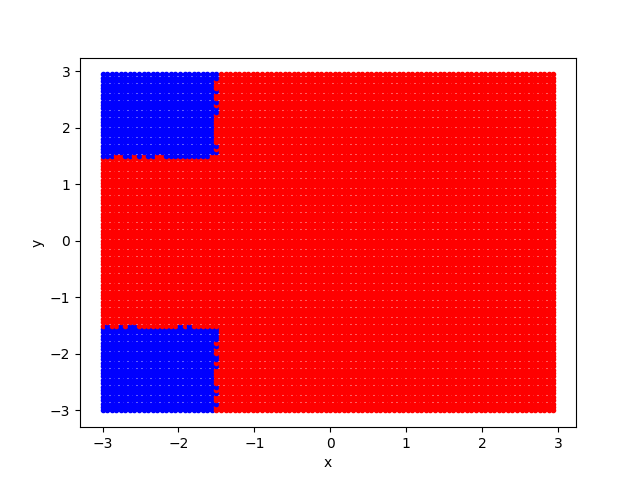
\includegraphics[scale=0.8]{p6.1a3}
	\subsection*{(a)}
		1-NN:\\
		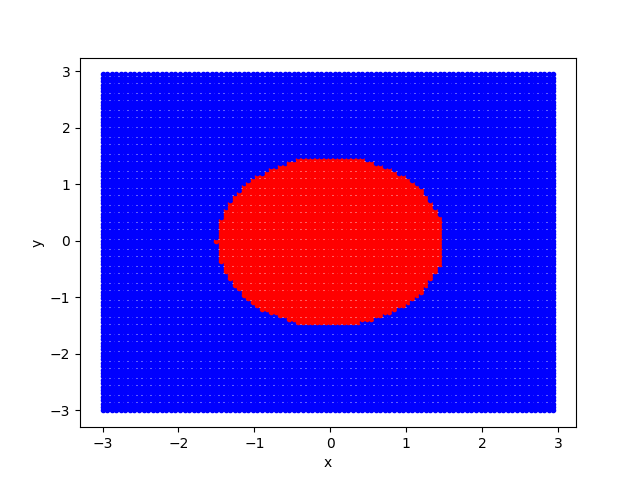
\includegraphics[scale=0.8]{p6.1b1}\\
		3-NN:\\
		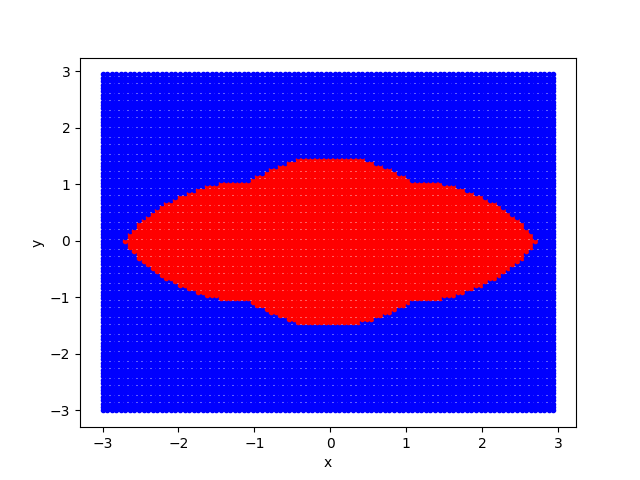
\includegraphics[scale=0.8]{p6.1b3}
		
	\section*{Problem 6.4}
		Note: same as Problem 6.1\\
		1-NN:\\
		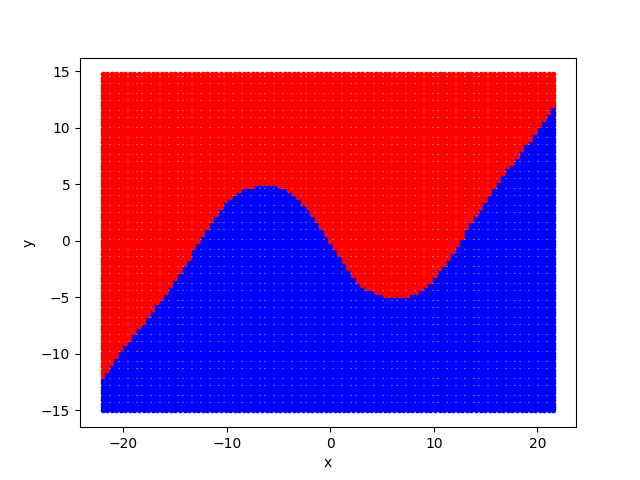
\includegraphics[scale=0.8]{p6.4a}\\
		3-NN:\\
		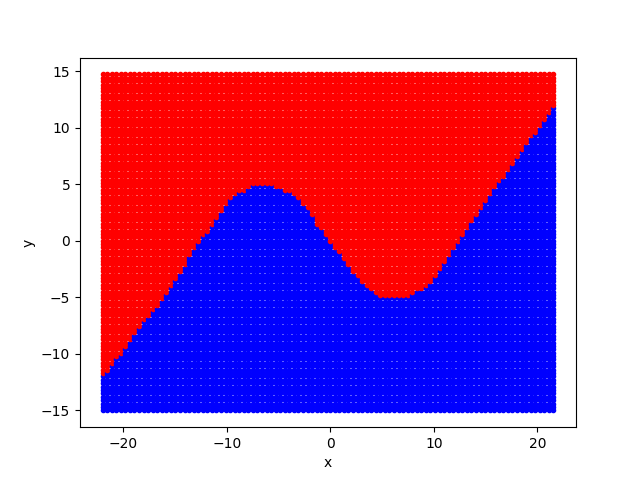
\includegraphics[scale=0.8]{p6.4b}
		
	\section*{Problem 6.16}
	\subsection*{(a)}
		Branch and bound took 1198 ms.\\
		Brute force took 26788 ms.
	\subsection*{(b)}
		Branch and bound took 1233 ms.\\
		Brute force took 26708 ms.
	\subsection*{(c)}
		For sufficiently large number of data points stored, branch and bound runs way faster.
	\subsection*{(d)}
		No. It only depends on the number of data points used in learning because in branch and bound, we don't need to look over all of them to classify each test point. The runtime can't be better than linear in the number of test points because we have to look over all of them to classify each.
\end{document}